\section{Introduction}
\label{lab3-Introduction}

For a penetration tester, it is essential to have both theoretical knowledge and
practical experience to succeed. This is why Threat Evaluation is considered an
important aspect of penetration testing, as it builds up the knowledge gathered
from the past exploits to mitigate future ones. The MITRE ATT\&CK
framework is a collection of adversary tactics and techniques based on
real-world examinations. It can give an understanding of what adversaries do in
an attack and what a defender must prioritise to defend against it.

\section{Task 1}
\label{lab3-Task1}
In this task, we will design three hypothetical vulnerabilities using a CVSS
score.

\subsection{JSON Web Token (JWT) Vulnerability}
\label{lab3-JWT}

A JWT is very often used to authenticate users through previously produced
tokens. It is encoded as an object that is digitally signed using JWS or
encrypted using JWE\@. On JWT.IO, it is easily possible to understand the
structure of a token and distinguish between portions of header, payload, and
verify signature. The header contains the signature or encryption algorithm and
the type of token.
\begin{figure}[H]
  \centering
  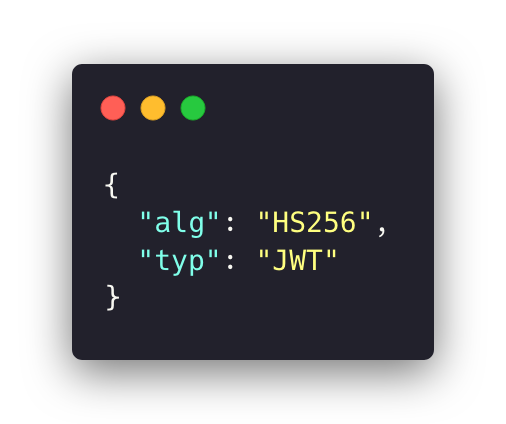
\includegraphics[width=0.4\textwidth]{figures/code/jwt-header}
  \caption{JWT Header}
  \label{f:jwt-header}
\end{figure}
The payload contains the claims about a user and more data related to it.
\begin{figure}[H]
  \centering
  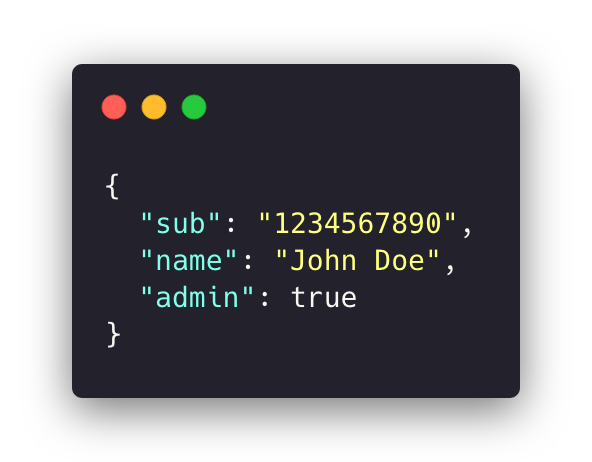
\includegraphics[width=0.3\textwidth]{figures/code/jwt-payload}
  \caption{JWT Payload}
  \label{f:p}
\end{figure}
And finally we have the signature that is used to verify the integrity and the
confidentiality.
\begin{figure}[H]
  \centering
  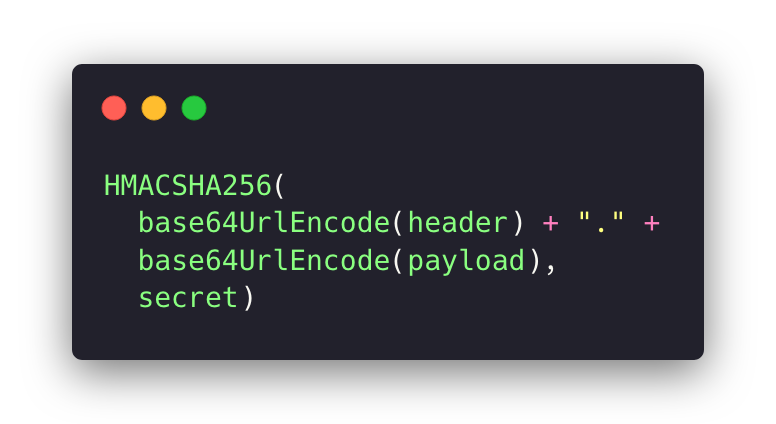
\includegraphics[width=0.4\textwidth]{figures/code/jwt-signature}
  \caption{JWT Signature}
  \label{f:jwt-signature}
\end{figure}
All these three parts together, in its compact JWT form are found in a
\lstinline{xxxxx.yyyyy.zzzzz} format where xxxxx is the header, yyyyy is the
payload and zzzzz is the signature.

The vulnerability involves a JWT with the header section containing the Hashed
Message Authentication Codes, allowing attackers to gain admin access through
the payload with an \lstinline{is_admin} field with a \lstinline{true} value.

\begin{description}[align=left]
  \item [Base Score: 8.7]
  \item [Attack Vector (Network):] the user sends the signed jwt token to the
  server
  \item [Attack Complexity (High):] the user needs a highly understanding of
  how the JWT structure works, the algorithms and authentication system
  \item [Privileges Required (None):] there are no specific needed privileges
  \item [User Interaction (None):] there is no other user interaction a part
  from the attacker
  \item [Scope (Changed):] this exploit can cause disrupt and changes to its
  target assets
  \item [Confidentiality (High):] the attack will have access to personal
  informations of a targetted user, meaning that the confidentiality is totally
  compromised.
  \item [Integrity (High):] similarly to the confidentiality section, the
  attacker will have access to the target information but also be able to change
  it, meaning that the integrity is compromised as well.
  \item [Availability (None):] since it's usually required access to the
  personal email to change password, we can assume that the availability is not
  compromised.
\end{description}

\subsection{Backdoor TCP}
\label{lab3-backdoor}
The following backdoor allows TCP remote access due to a system script that has
been found for all debian distributions.

\begin{description}[align=left]
  \item [Base Score: 9.8]
  \item [Attack Vector (Network):] the backdoor is accessed through the
  network as the attacker will be connecting remotely
  \item [Attack Complexity (Low):] the complexity of the attack is relatively
  low as there are exploits that would function similarly and there is vast
  knowledge and resources available on the internet
  \item [Privileges Required (None):] no privileges are required
  \item [User Interaction (None):] user interaction is unnecessary because the
  backdoor is in a system file that starts at every boot
  \item [Scope (Unchanged):] the scope is unchanged as the backdoor provides
  access only to a given session.
  \item [Confidentiality (High):] since the attacker will have complete
  control, we can assume that confidenciality is compromised.
  \item [Integrity (High):] integrity is compromised as the attacker will have
  read/write access to all the files in the system.
  \item [Availability (High):] the attacker can decide to limit the user
  interactivities and cut him off completely, meaning that also availability
  will be compromised.
\end{description}

\subsection{SQL Injection}
\label{lab3-sql}
An attacker can inject SQL commands into a web application meaning that he can
gain access to sensitive information and query manipulation. This attack can be
performed on any SQL database and web services are a common target. The attacker
could get privileges and be able to delete, create and modify tables.

\begin{description}[align=left]
  \item [Base Score: 8.6]
  \item [Attack Vector (Network):] the attacker will be sending the SQL
  command to the server through the network
  \item [Attack Complexity (Low):] the complexity could be higher, but since
  the knowledge of this technique is very spread around the internet, it is not
  the case anymore
  \item [Privileges Required (None):] no privileges are required
  \item [User Interaction (None):] user interaction is unnecessary, the
  attacker will be the only one needed.
  \item [Scope (Unchanged):] this exploit can cause disrupt and changes to its
  target assets
  \item [Confidentiality (High):] the attack will have access to personal
  informations of a targetted user, meaning that the confidentiality is totally
  compromised.
  \item [Integrity (High):] integrity is compromised as the attacker may
  change the items in the table.
  \item [Availability (High):] the availability is compromised as the attacker
  could destroy the database and users may not be able to access their accounts
  or other services related to it.
\end{description}

\newpage
\section{Task 2}
\label{lab3-Task2}
This task asks to name all categories of enterprise tactics and their unique
identifiers that starts from TA\@. We will then describe three of them using the
template given.

\begin{table}[h!]
  \begin{center}
    \label{tab:table1}
    \begin{tabular}{c c}
      \toprule
      \textbf{Enterprise Tactic} & \textbf{Pre-ATT\&CK Tactics} \\
      \midrule
      TA0043 & TA0012\\
      TA0042 & TA0013\\
      TA0001 & TA0014\\
      TA0002 & TA0015\\
      TA0003 & TA0016\\
      TA0004 & TA0017\\
      TA0005 & TA0018\\
      TA0006 & TA0019\\
      TA0007 & TA0020\\
      TA0008 & TA0021\\
      TA0009 & TA0022\\
      TA0011 & TA0023\\
      TA0010 & TA0024\\
      TA0040 & TA0025\\
      \bottomrule
    \end{tabular}
  \end{center}
\end{table}

\subsection{T1595 Active scanning}
\label{lab3-tactics}
Unlike passive scanning, which is more of an observer storing information seen,
active scanning actively searches for information by interacting with the
network. An excellent example of this would be Arp-scan.
  \begin{description}[align=left]
    \item [Unique Identifier:] T1595
    \item [Platforms Affected:] PRE Matrix
    \item [Permissions Required:] none
    \item [Procedure Examples:] ARP-scan bombards the network of Arp request
    to see what machine answered and then display the Ip and mac address and
    vendor of the machine who answered; this is active due to the interaction
    with the network.
    \item [Mitigation Technique:] there is no specific mitigation technics
    this is not easily mitigated since it is based on behaviour and outside the
    enterprise scope; limiting any leaks or sensitive data in the wild is the
    best defence in this case.
    \item [Detection Technique:] there are no specific detection technics,
    but since it is behaviour based on network behaviour analysis that could
    help, encryption and blacklisting could also be used.
  \end{description}

\subsection{T1543 Create or modify system process}
\label{lab3-tactics2}
In order to add persistence to a payload, one might obfuscate it by hiding it in
or as a System Process given the fact that they are loads of System processes
and that most of them start at boot up no one would notice a new service or
malicious code hiding in a service.
  \begin{description}[align=left]
    \item [Unique Identifier:] T1543
    \item [Platforms Affected:] Linux, Windows, macOS
    \item [Permissions Required:] root or admin privilege
    \item [Procedure Examples:] Exaramel for Linux ID:S0401
    \item [Mitigation Technique:] M1033 Limit Software Installation
  \end{description}

  \subsection{T1055 Process Injection}
  \label{lab3-tactics3}
Process injection is the ability to run code in address space from other
processes.
    \begin{description}[align=left]
      \item [Unique Identifier:] T1055
      \item [Platforms Affected:] Linux, Windows, macOS
      \item [Permissions Required:] none
      \item [Procedure Examples:] S0469 ABK ability to inject shellcode
      into svchost.exe
      \item [Mitigation Technique:] M1033 Limit Software Installation
    \end{description}

\newpage
\section{Task 3}
\label{lab3-Task3}
In this task, we will scan the network hosts within the scope and identify
available services provided by the hosts and identify the software version of
these services. On a side note, we included only the IPs in the list only if
there was a version of the service available.\\

\begin{table}[h!]
  \begin{center}
    \label{tab:table2}
    \begin{tabular}{c c c}
      \toprule
      \textbf{IP} & \textbf{Service} & \textbf{Version} \\
      \midrule
      192.168.69.110 & ssh & OpenSSH 8.3\\
      192.168.69.113 & ssh & OpenSSH 7.6p1\\
      192.168.69.119 & ssh & OpenSSH 5.3p1\\
      & http & Apache 2.2.14\\
      & netbios & Samba 3.X-4.X\\
      & imap & Courier Imap\\
      & ssl/http & Apache 2.2.14\\
      & java-object & Java Object Serialization\\
      & http & Apache Tomcat 1.1\\
      & http & Jetty 6.1.25\\
      192.168.69.123 & msrpc & Microsoft Windows RPC\\
      & netbios & Microsoft Windows Netbios SSN\\
      & Microsoft ds & Windows 7 7601\\
      192.168.69.124 & ssh & OpenSSH 8.3\\
      192.168.69.127 & Ipp & CUP 1.1\\
      192.168.69.166 & ssh & OpenSSH 8.3\\
      & http & Apache 2.2.14\\
      192.168.69.177 & ssh & OpenSSH 5.9p1\\
      192.168.69.179 & Msrpc & Microsoft Windows RPC\\
      & Netbios SSN & Netbios SSN\\
      192.168.69.200 & ssh & OpenSSH 8.3\\
      \bottomrule
    \end{tabular}
  \end{center}
\end{table}

\subsection{OpenSSH Vulnerabilities}
In the list below, some of the vulnerabilities related to OpenSSH and its
various versions.
\begin{description}[align=left]
  \item [CVE-2020-15778:] Allows command injections. In order to use this
  exploits, the attacker also need social engineering or directly manipulate a
  system administration
  \item [CVE-2020-14145:] Allows man in the middle attacks. It is required to
  have control of a DNS or network
  \item [CVE-2020-1292:] This vulnerability allows for privilege elevation and
  it's a consequence of Windows misconfiguration
  \item [CVE-2019-7639:] Allows the attacker to login with wrong login details
  even though the failure is even logged in the system
\end{description}

\subsection{Apache Vulnerabilities}
In the list below, some of the vulnerabilities related to Apache and its
various versions.
\begin{description}[align=left]
  \item [CVE-2009-3555:] Allows for man in the middle attack through an error
  that occurs when TSL protocol is working
  \item [CVE-2010-0425:] Allows attackers to remotely execute custom code. It
  leverages the isapi module in win32
  \item [CVE-2010-1312:] Allows attackers to inspect HTTP requests undetected.
  \item [CVE-2015-1833:] Allows attackers to read files and send requests to
  intranet
  \item [CVE-2009-2699:] Allows attackers to perform Denial of Services via
  unspecified HTTP requests
\end{description}

\subsection{Jetty Vulnerabilities}
In the list below, some of the vulnerabilities related to Jetty and its
various versions.
\begin{description}[align=left]
  \item [CVE-2009-3555:] Attacker can craft URIs using encoded characters in
  order to access and bypass security
  \item [CVE-2021-28165:] Allows the attacker to compromise availability
  through CPU usage
\end{description}

\section{Conclusion}
\label{lab3-conclusion}
In this lab, I have learned that evaluating threats and vulnerabilities is
essential for a penetration tester. I have enjoyed creating hypothetical
vulnerabilities and navigating the CVE Mitre website to research vulnerabilities
scanned in the network. I feel like it could be split into two labs as it was
very time consuming, but overall an entertaining experience!
